\documentclass[review]{elsarticle}

\usepackage{lineno,hyperref}
\modulolinenumbers[5]
%\linenumbers

\usepackage{numcompress}\bibliographystyle{model4-names}\biboptions{authoryear}

%\documentclass[a4paper,donotrepeattitle,fleqn]{cas-dc}
%\documentclass[a4paper,fleqn]{cas-dc}
\usepackage{graphicx}
\graphicspath{ {./images/} }
\usepackage{makecell}
\usepackage{algorithmic,algorithm2e}
%\usepackage[ruled,vlined,linesnumbered]{algorithmic,algorithm2e}
\usepackage{lscape}
%From Table
%\usepackage{makecell}
%\usepackage{xcolor}
%From Footnot and HyperLinks
%\usepackage[pdftex]{hyperref}
%From Equations
%\usepackage{amsmath}
\usepackage{tcolorbox}
%\usepackage[numbers]{natbib}
%
%\usepackage{natbib}
%\bibliographystyle{abbrvnat}
%
%\usepackage{numcompress}\bibliographystyle{model4-names}
%\biboptions{authoryear}
%%%Author definitions
%\def\tsc#1{\csdef{#1}{\textsc{\lowercase{#1}}\xspace}}
%\tsc{WGM}
%\tsc{QE}
%\tsc{EP}
%\tsc{PMS}
%\tsc{BEC}
%\tsc{DE}
%%%

\begin{document}
%\begin{frontmatter}
%\let\WriteBookmarks\relax
%\def\floatpagepagefraction{1}
%\def\textpagefraction{.001}
%\shorttitle{Multi-core Synthesis of Solar PV systems.}
%\shortauthors{E. Galvão, A. Trindade and L. Cordeiro.}

\title {Multi-core synthesis and maximum satisfiability for optimal sizing of solar photovoltaic systems.}                      
%\tnotemark[1,2]

%\tnotetext[1]{This document is the results of the research
%   project funded by the National Science Foundation.}

%\tnotetext[2]{The second title footnote which is a longer text matter
%   to fill through the whole text width and overflow into
%   another line in the footnotes area of the first page.}

\author[mymainaddress]{Edilson Galvão}

\author[mymainaddress]{Alessandro Trindade\corref{mycorrespondingauthor}}
\cortext[mycorrespondingauthor]{Corresponding author}
\ead{alessandrotrindade@ufam.edu.br}
%\ead[url]{www.elsevier.com}

\author[mysecondaryaddress]{Lucas Cordeiro}

%
\address[mymainaddress]{Federal University of Amazonas, Av. Rodrigo Octávio, 6200, 69077-000 Manaus-AM-Brazil}
\address[mysecondaryaddress]{University of Manchester, Kilburn Building, Manchester M13 9PL}
%
%
%
%\author[1]{Edilson Galvão}
%\author[1]{Alessandro Trindade}[orcid=0000-0001-8262-2919]
%\ead{alessandrotrindade@ufam.edu.br} 
%\cormark[1]
%\author[2]{Lucas Cordeiro}[orcid=0000-0002-6235-4272]

% Corresponding author indication

%\affiliation[1]{organization={Federal University of Amazonas, Department of Electricity},
%            addressline={Av. General Rodrigo Octavio, 1200 - Coroado I}, 
%            city={Manaus},
%            postcode={69077-000}, 
%            state={Amazonas},
%            country={Brazil}}
%\cortext[1]{Corresponding author}
%\affiliation[2]{organization={The University of Manchester, Department of Computer Science},
%            addressline={Oxford Rd}, 
%            city={Manchester},
%            postcode={M13 9PL}, 
%            country={United Kingdom}}
%
%\address[1]{Federal University of Amazonas, Department of Electricity, Av. General Rodrigo Octavio, 1200 - Coroado I, Manaus - AM, Brazil}
%\address[2]{The University of Manchester, Department of Computer Science, Oxford Rd, Manchester M13 9PL, United Kingdom}

%\cormark[1]
%\fnmark[1]
%\ead{cvr_1@tug.org.in}
%\ead[url]{www.cvr.cc, cvr@sayahna.org}

%\credit{Conceptualization of this study, Methodology, Software}

%\author[2,4]{Alessandro Trindade}%[style=chinese]

%\author[2,3]{CV Lucas Cordeiro}[%
%   role=Co-ordinator,
%   suffix=Jr,
%   ]
%\fnmark[2]
%\ead{cvr3@sayahna.org}
%\ead[URL]{www.sayahna.org}

%\credit{Data curation, Writing - Original draft preparation}

%\address[2]{Av. General Rodrigo Octavio, 1200 - Coroado I, Manaus - AM, Brazil}

%$$\author%
%$[1,3]
%${Rishi T.}
%$\cormark[2]
%$$\fnmark[1,3]
%$\ead{rishi@stmdocs.in}
%$\ead[URL]{www.stmdocs.in}

%$\address[3]{ Oxford Rd, Manchester M13 9PL, United Kingdom}

%\cortext[cor1]{Corresponding author}
%\cortext[cor2]{Principal corresponding author}
%\fntext[fn1]{This is the first author footnote. but is common to third
%  author as well.}
%\fntext[fn2]{Another author footnote, this is a very long footnote and
%%  it should be a really long footnote. But this footnote is not yet
%  sufficiently long enough to make two lines of footnote text.}

%\nonumnote{This note has no numbers. In this work we demonstrate $a_b$
%  the formation Y\_1 of a new type of polariton on the interface
%  between a cuprous oxide slab and a polystyrene micro-sphere placed
%  on the slab.
%  }

\begin{abstract}
Energy consumption forecasting growth for the world is $1.3$\% until $2040$, and solar photovoltaic systems had the highest adoption as an alternative for fossil fuels. To improve the optimal sizing of stand-alone systems, we develop an automated formal synthesis technique for stand-alone systems. Our approach, named PVz, is based on the counterexample-guided inductive synthesis; it has a multi-core feature, which can obtain optimal sizing of photovoltaic systems focusing on life cycle cost analysis. Starting with the electrical demands of a house, our technique seeks a set of electrical equipment to find the best possible combination of devices: a combination of electrical compatibility with the global lowest price, based on a 20-years horizon of operation and maintenance. We present our experimental results based on seven case studies, Targeting to validate and compare our results, we obtained the optimal sizing from a commercial optimization tool for the same case studies and submitted each designed system to a popular simulation tool. We conclude that our approach provides more accurate results than existing literature approaches and with impressive time to respond compared with the previous automatic synthesis techniques.

%\noindent\texttt{\textbackslash begin{abstract}} \dots 
%\texttt{\textbackslash end{abstract}} and
%\verb+\begin{keyword}+ \verb+...+ \verb+\end{keyword}+ 
%which contain the abstract and keywords respectively. 

%\noindent Each keyword shall be separated by a \verb+\sep+ command.
\end{abstract}

%\begin{graphicalabstract}
%\includegraphics{figs/grabs.pdf}
%\end{graphicalabstract}

%\begin{highlights}
%\item Research highlights item 1
%\item Research highlights item 2
%\item Research highlights item 3
%\end{highlights}

\begin{keyword}
formal synthesis\sep software verification\sep model checking\sep solar photovoltaic systems
%quadrupole exciton \sep polariton \sep \WGM \sep \BEC
\end{keyword}

%\end{frontmatter}

\maketitle

\section{Introduction}
Recent studies on global energy indicate that $789$ million people have no access to electricity, which is $10$\% of the world population \citep{Energyprogressreport}. From $2010$ until $2018$, the effort to reduce the number of people without electricity access increased, and the results are positive. Quantitatively the result was a decrease from $1.2$ billion to $0.84$ billion people without electrical energy. Out of this total, renewable energy solutions are responsible for $136$ million people receiving basic energy service as shown in \cite{Energyprogressreport}. However, lack of access to clean and affordable energy is considered a core dimension of poverty \citep{Hussein2012}; and a direct impact is a low Human Development Index (HDI) \citep{Coelho}. 

Decentralized or distributed systems, as solar photovoltaic (PV) in stand-alone and mini-grid systems, are indicated to be the lowest-cost solution for 75\% of the connections required in the world~\citep{Hussein2012}. This is confirmed by the in the result of renewable energy reported by the global bank, where 17.3\% of global energy is based on wind and solar energy~\citep{Energyprogressreport}.  

Note that changes to improve the electrical energy usage requires us to reason over the PV model: the more precise sizing for electrical grids or stand-alone systems, the more meaningful the use of renewable energies. For this purpose, there are tools available in the market; some of them are created for general-purpose such as MATLAB~\citep{Benatiallah2017} and others for specific electrification studies like RETScreen, and HOMER~\citep{Pradhan,Swarnkar}. However, industrial applications require the design solution to be optimum, considering equipment manufacturers and models available on the market and not minimum or maximum values of current or power for the optimized items~\citep{DBLP:journals/corr/abs-1909-13139, Applasamy2011}. We must evaluate the electrical compatibility among the equipment, which can only be achieved with specialized PV optimization software. To summarize, an optimal solution means that the lowest cost for the equipment list meets the electrical design requirements.
 

Given the above, the HOMER tool delivers an optimal solution in a smaller scope, where only batteries and solar panels are optimized while all other modules are simulated. In contrast, the technique described in this work, named PVz, is capable of optimizing, in addition to solar panels and batteries, electrical inverters, and controllers. Furthermore, the clear difference between the optimized electrical devices ensures greater correctness once both techniques are compared, favoring a more extensive design-space coverage.

Here, we have developed a variant of the Counterexample Guided Inductive Synthesis (CEGIS)~\citep{AbateCAV2018} for synthesizing optimal sizing of stand-alone PV systems using commercial equipment data. 

We used a solver called Z3~\citep{BjornerPF15}. Internally, the Z3 tool contains a module to include optimization objectives. This module is named $\nu$Z and integrates state-of-the-art algorithms for optimization and extra tools to solve linear restriction problems. Our technique synthesizes a complete design solution for stand-alone PV systems in each iteration, but it is not sure it is the lowest global cost. Thus, the candidate solution passes through an SMT solver to reduce the number of possible states.  Note that each iteration can be lower or higher than the current reference, once found a value lower than the current reference, and it respects the user constraints. The reference is updated globally. If the verification by the SMT solver step fails, then there is an optimal solution. Thus, all content produced is saved as a counterexample with an optimal sizing that meets both power reliability and system cost. If the verification step does not fail, the content produced is ignored. The main originality of our work relies on a practical approach to pursuing the optimal solution of PV systems using formal methods. 
 
It is challenging to find studies based on state-of-the-art solvers as ESBMC~\citep{esbmc2018}, CPAchecker~\citep{Beyer2011} and Z3~\citep{BjornerPF15}. Therefore, the starting point for this work~\citep{VSTTE2020, TrindadeCordeiro19, AraujoBCF16} are studies that derive from the year $2019$ and converge to analyze the optimization problem of photovoltaic systems using SMT solvers and commercial tools such as HOMER and PVsyst. 

\noindent \textbf{Contributions.} This paper makes the following original contributions. First, it is a radical improvement in the base paper's performance describing formal synthesis for stand-alone PV system application~\citep{DBLP:journals/corr/abs-1909-13139}. Second, the technique described here supports data processing parallelization since it relies on a multi-core processor. Third, the state space coverage was increased compared to the base article~\citep{VSTTE2020}. It was possible to cover and compute all the spaces of the combinations of electrical equipment. Fourth, experimental results with seven case studies show that the formal synthesis approach qualitatively outperforms an existing state-of-the-art optimization tool. Lastly, the results are validated with accurate commercial design software called PVsyst.

\noindent \textit{Outline}. The remainder of this paper is organized as follows. Section~\ref{sec:Background} shows how to perform traditional and synthesized sizing of PV systems. Section~\ref{sec:Synthesis} details our proposed technique in comparison with traditional CEGIS technique. Section~\ref{sec:sizing} explains the components and how to size stand-alone solar PV systems. The details of our algorithms and the construction of our PVz tool is presented in section~\ref{sec:SynthesizingOptimalSolarPhotovoltaicSystems}. Section~\ref{sec:results} is devoted to the results. Section~\ref{sec:Conclusions} presents the conclusion and describes future work.

%-----------------------------------------------------------
\section{Background}
\label{sec:Background}
%-----------------------------------------------------------
Fig.~\ref{fig:optimization} illustrates how to obtain the optimal sizing of a stand-alone PV system using two modes. The first one is the traditional model called \textit{\textbf{traditional sizing}}, which includes manual verification by computing the electrical equipment capacity and installation for validation. Concerning the first mode, there are still commercial tools as MATLAB~\citep{Benatiallah2017} and HOMER~\citep{Pradhan,Swarnkar}, which simulate the real electrical system. The second includes \textbf{\textit{automated synthesis}} that encompasses verification engines. This option proves viable since it generates more complex and accurate data than the traditional way described previously. 

For \textbf{input} data, we can consider weather data, price information about each piece of equipment, design requirements, load curve, power demand, and design assumptions. This information is converted into a matrix of data and exposed as global content to the software.

For the \textbf{output} data and a more straightforward reading of this work, we will assume from now on that every benchmark that contains a valid answer will be called \textbf{satisfiable (SAT)}. By contrast, when there is no solution, we will call it \textbf{unsatisfiable (UNSAT)}. If there is a set of renewable energy equipment, which can be combined (price and system hardware composition), the result is SAT.

\begin{figure}[ht]
\begin{center}
\fbox{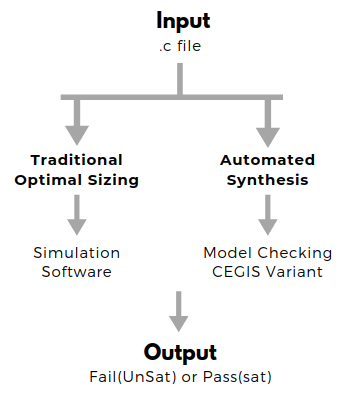
\includegraphics[width=0.5\textwidth]{TraditonalVsAutoFlow.png}}
\end{center}
\caption{Comparative image of the traditional method versus the proposed method.}
\label{fig:optimization}
\end{figure}
  
The automated synthesis technique is mathematical reasoning about a formal model, where the SAT result is a counterexample. The counterexample is intended to record changes in the values of the program variables during program execution. In this work, since the system's answer is SAT, the counterexample will show the status of all variables when the solution was found. Thus, the answer can guide the software or client to choose the best combination of electrical machines. However, the traditional way does not offer the quantity of necessary data about the system and internal modes ~\citep{Benatiallah2017,Pradhan,Swarnkar}. Another notable topic that must highlight is each model's coverage; models that use Automated Synthesis (via BMC engines) can ensure complete coverage over the entire state-space, instead of local states as a traditional model.

%-----------------------------------------------------------
\section{Program Synthesis}
\label{sec:Synthesis}
%-----------------------------------------------------------

The essence behind program synthesis is to automatically build a $P$ program that satisfies a correctness specification $\sigma$ automatically by engines using a correctness specification $\sigma$. In particular, we consider $\sigma$ as a starting point, and then we incrementally produce a sequence of candidate solutions that partly satisfy it~\citep{Abateetal2017}. As a result, a given candidate program $p$ is iteratively refined to match $\sigma$ more closely. Figure~\ref{Counter-Example-Guided-Inductive-Synthesis} illustrates the architecture described here.

%
\begin{figure}[ht]
\begin{center}
\fbox{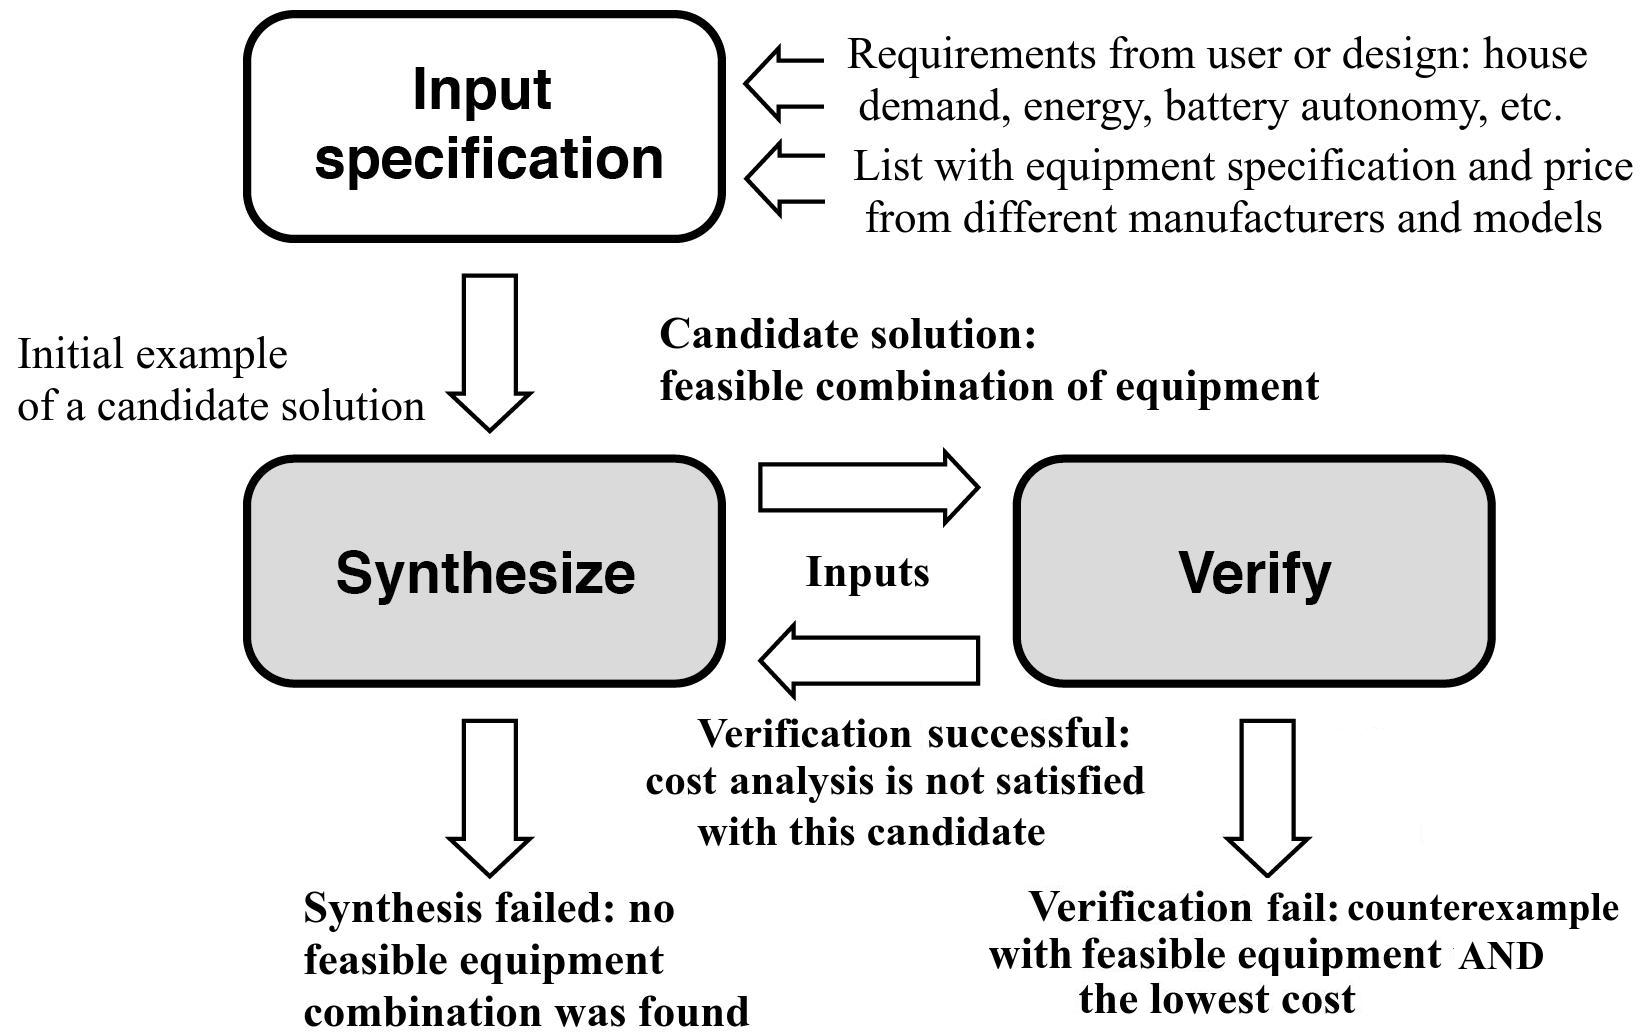
\includegraphics[width=0.7\textwidth]{fig2_rev2.jpg}}
\end{center}
	\caption{CEGIS in PV system sizing.}
	\label{Counter-Example-Guided-Inductive-Synthesis}
\end{figure}

$\sigma(\vec{x}, \vec{F})$, where $\vec{F}$ ranges over functions, $\vec{x}$ ranges over ground terms. On the one hand, SMT solvers usually support the quantifier-free (QF) formula of $\sigma$. On the other hand, the ground terms are interpreted over some finite domain $\mathcal{D}$. The specification for PV system includes house demand in Watt, electrical energy (kWh), and battery autonomy in hours; it is demanding to provide a list of equipment and price.

In Figure~\ref{Counter-Example-Guided-Inductive-Synthesis}, the phases {\sc Synthesize} and {\sc Verify} interact via a finite set of test vectors {\sc inputs}, which is incrementally updated. Given the correctness specification $\sigma$, the {\sc Synthesize} procedure tries to find an existential witness $\vec{F}$ satisfying the specification $\sigma(\vec{x}, \vec{F})$, for all $\vec{x}$ in {\sc inputs} (as opposed to all $\vec{x} \in \mathcal{D}$). If {\sc Synthesize} succeeds in finding a witness~$\vec{F}$, the found vector {\sc inputs} can be considered as one possible candidate solution to the full synthesis formula, which is then passed to {\sc Verify} phase to check whether it is a proper definitive solution ({\it i.e.}, $\vec{F}$ satisfies the specification $\sigma(\vec{x}, \vec{F})$ for all $\vec{x}\in\mathcal{D}$)~\citep{iet-cps.2018.5006}. If this step occurs, it means that the algorithm finished the process. 

Each iteration of the traditional CEGIS loop adds a new input to the finite set {\sc inputs}, and this updated set is used for synthesis. The full set of inputs $\mathcal{D}$ is finite because we use bit-vector expressions, thus, the refinement loop can iterate only over a finite number of times. However, the {\sc Synthesize} phase may conclude that there is not a candidate solution complying with $\sigma$ for the finite set of {\sc inputs}.

Related to our proposed CEGIS variant, there exist four differences related to the traditional CEGIS:
(1) there is no test vector. Therefore, every candidate is generated in the {\sc Synthesize} phase and sent to the {\sc Verify} phase; 
(2) if the {\sc Verify} phase is unsuccessful, a new candidate is generated by {\sc Synthesize} and 
(3) the lower bound of the {\sc Verify} phase is incremented to search for the lowest cost; as a result,
(4) there exists no refinement from the {\sc Verify} phase back to the {\sc Synthesize} step. More specifically, a new counterexample is not added to the {\sc input} set since a failure during the {\sc Verify} phase will only discard a given candidate, which can be feasible in the next iteration since a new lower bound is assumed.

In summary, our proposed technique is based on CEGIS and aims to synthesize the optimal solution for autonomous photovoltaic systems through optimization techniques.

%-----------------------------------------------------------
\section{Sizing Stand-alone Solar PV Systems}
\label{sec:sizing}
%-----------------------------------------------------------
A PV system is illustrated in Fig.\ref{fig:blockdiagram}. It employs the PV generator (\textit{panel or an array}), a semiconductor device that can convert solar energy into DC electricity. We hold \textit{batteries}, where power can be stored and used for night hours or rainy days. The use of batteries demands the use of a \textit{charge controller}~\citep{Hansen}. The PV arrays produce direct current (DC), and as our homes use alternating current (AC), thus an \textit{inverter} is required (DC/AC converter)and therefore, when the PV system contains an AC load, a DC/AC conversion is required. The \textit{AC load} govern the behavior of the PV system.
%
\begin{figure}[ht]
\fbox{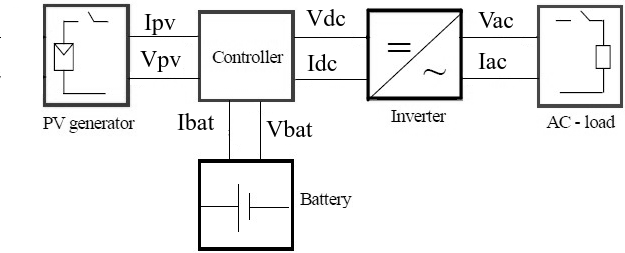
\includegraphics[width=0.6\textwidth]{blockdiagramPVS2_rev.png}}
\centering
\caption{Block diagram for a typical stand-alone PV system~\citep{Hansen}.}
\label{fig:blockdiagram} 
\end{figure}
 
The sizing check phase can ensure that the system meets the sizing steps related to the critical period method (worst month) for solar photovoltaic design~\citep{Pinho}. The adoption of MPPT (Maximum Power Point Tracking) charge controller is based on the improvements in energy generation and the availability in the market. 
 
At this paper, we adopted a higher-level explanation about PV sizing, whose process is detailed online.\footnote{\href{https://cutt.ly/Dz1Ua6Q}{https://cutt.ly/Dz1Ua6Q}} 
Fig.~\ref{fig:flow} illustrates an overview of the steps that must be taken to size a stand-alone PV system.
%
\begin{figure}[ht]
\fbox{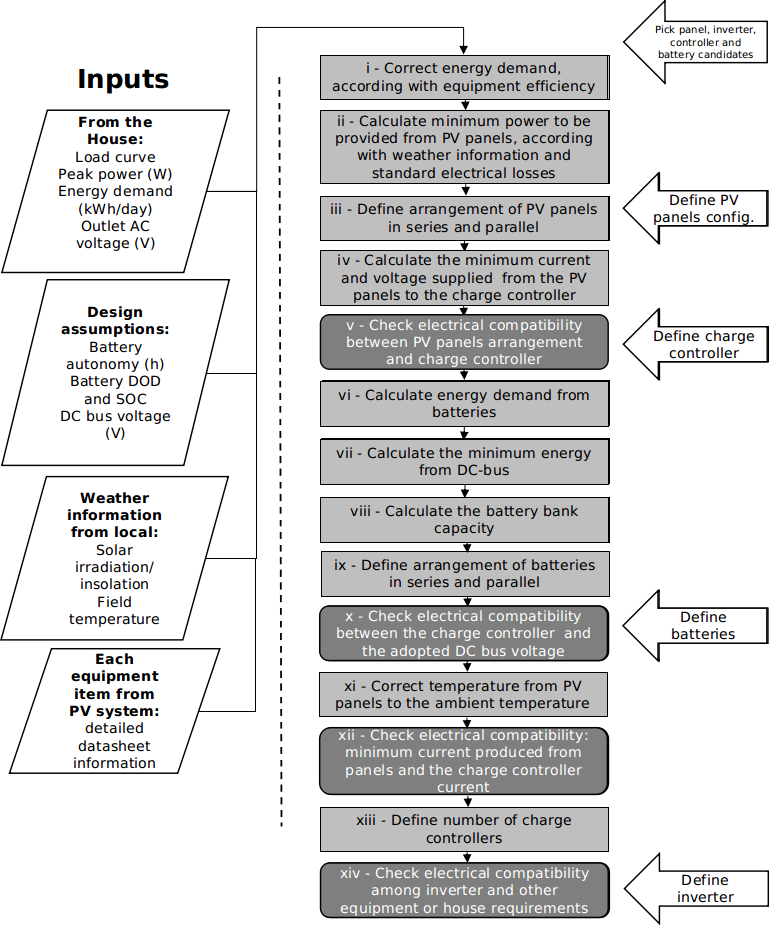
\includegraphics[width=0.7\textwidth]{flowchart.png}}
\centering
\caption{High level description of stand-alone PV system sizing process.}
\label{fig:flow} 
\end{figure}
 

On the left side of Fig.~\ref{fig:flow}, we describe the needed \textbf{inputs} to size a PV system. There are electrical demands from the house; there are design assumptions, weather information from the site of the PV system deployment, and a list of equipment to cover the components listed in Fig.~\ref{fig:blockdiagram}. It is possible to use or not a commercial equipment list. Nevertheless, if the decision is to use fictional equipment specifications, we can cause an electrical incompatibility among items when the real one is deployed in the field.
 
There exist steps for calculation of some variables to deal with the specification of each item of equipment, including electrical issues and quantitative issues enumerated from \textbf{i} to \textbf{xiv} in Fig.~\ref{fig:flow}; those represent different shades of gray of the rectangle boxes. The process starts with a candidate list of PV panels, charge controller, batteries, and inverter, as indicated in the flowchart—broad arrows on the right side show where an item is completely defined in the sizing process. The diagram does not show the returning paths. However, if the candidate item is not electrically compatible or does not meet some electrical demands, it is changed during the search for optimal sizing. The last box checks the inverter's compatibility between the DC-bus voltage and the outlet's required AC voltage. The inverter power must be lower than the charge controller power to avoid overcharge. All the items are defined at the end of the flowchart, and PV sizing is finished.

These equations model the PV system's continuous-time behavior; they produce real numbers, except for the batteries and panels. Real numbers are converted into integer ones, regarding the minimum or maximum according to each equation. The verification and simulation tools must handle non-linear real arithmetic to produce the correct result. Our mathematical model uses floating-point arithmetic, which is an approximation of real numbers. However, this is not an issue based on the magnitude of the physical quantities and the variables adopted~\citep{DBLP:journals/corr/abs-2004-12699}.


%------------------------------------------------------
\section{Synthesizing Optimal Sizing of Stand-alone Solar Photovoltaic Systems}
\label{sec:SynthesizingOptimalSolarPhotovoltaicSystems}
%------------------------------------------------------
The best fit between the two objectives is how we obtain optimal sizing for PV systems: \textit{power reliability} and \textit{system cost}~\citep{Alsadi2018}. Our study is based on the critical period solar energy method~\citep{Pinho}, as described in Section~\ref{sec:sizing}. Furthermore, we use an adapted Life Cycle Cost (LCC) analysis, where the acquisition cost of every item of equipment is considered, besides the installation cost, the operational and maintenance costs~\citep{Alsadi2018}; theses costs are represented by Equation~\ref{eq:LCC}.
%
\begin{equation}
\label{eq:LCC}
LCC = EC + EM
\end{equation}
%
\noindent EC denotes the costs of the following equipment: $C_{PV}$ is the PV array cost, $C_{bat}$ is the initial cost of batteries, $C_{charger}$ is the cost of the charger, $C_{inv}$ is the inverter cost.
\begin{equation}
\label{eq:EquipamentCost}
EC = C_{PV} + C_{bat} + C_{charger} + C_{inv}
\end{equation}

EC denotes other costs related to the maintenance and proper functioning of the electrical system: $C_{installation}$ is the installation cost, $C_{batrep}$ is battery replacement cost at current prices, and $C_{PWO\&M}$ is operation and maintenance costs at current rates.
\begin{equation}
\label{eq:EquipamentMaintenence}
EM = C_{installation} + C_{batrep} + C_{PWO\&M}
\end{equation}

In this study, we will use a $C_{installation}$ equivalent to $5$\% of total equipment cost and a $C_{PWO\&M}$ equal to U\$ 289.64/year, according to Amazon State literature data~\citep{Agrener2013}; and an LCC lifetime analysis of $20$ years.

In this section, we will describe our algorithms and how model checking can be used as a back-end verification engine~\citep{DBLP:journals/corr/abs-1909-13139}. Algorithm~\ref{base_opt_code} describes how to save and expose the correct solutions and the optimal solution, and Algorithm~\ref{base_opt_code2} is responsible for verifying the mathematical assertion over electrical equipment.

\begin{algorithm}[ht]
\SetAlgoLined
\KwResult{returns a feasible sizing of PV system with the lowest cost }
Initialize arrays and variables\;
Create Satisfable List called NodeSatList\;
Create AllAvailableNodes list\;
Create maximumCost as a long variable\;
 \ForAll{AllAvailableNodes node}{
  isLowestNode = solve(node)\;
  \If{isLowestNode = true}{
 lock(this)\;
 maximumCost = node.cost\;
 NodeSatList.add(node)\;
 unlock(this)\;
   }
 }
\textbf{return} NodeSatList.OrderBy(x.Cost).FirstOrDefault()
\caption{Find by the optimal solution}
\label{base_opt_code}
\end{algorithm}

Algorithm~\ref{base_opt_code} receives as input the data described in Fig.~\ref{fig:optimization}. This content is represented in matrices and global variables. The first line includes the manufacturer's data, prices of PV panels, batteries, charge controllers, and inverters. Lines $2$, $3$, and $4$ represent the state-space, the nodes that satisfy the equations, and the lowest global cost.

\textit{AllAvailableNodes} is the data set representing the total sample of states to be explored; its purpose is to ensure $100$\% coverage of equipment combinations. A node represents a feasible arrangement or not of proposed electrical equipment for the test case; that is, among all the solutions and ways of organizing the photovoltaic system under study, a node corresponds to one possible solution. We have an object-oriented class that stores all relevant information. For example, electrical equipment that will be combined, the solar radiation level in the region, best global equipment cost, lowest local equipment cost, consumption, and electrical details of each test case) so that the solver can process the set of equipment and validate it.

The representation of the problem through nodes decreases the complexity of processing data in physical processor architectures that accept multi-threads. Therefore, the parallel loop is used to process each node separately. The function \textit{solve} described in Algorithm~\ref{base_opt_code2} returns true when the node is a possible solution, and the cost is lower than the global maximum cost. Therefore, the lock function was added to ensure the proper storage of results processed by many threads simultaneously. After the internal loop ends, the last action returns the optimal solution found in the list that contains all possible solutions.

\begin{algorithm}[ht]
\SetAlgoLined
\KwResult{Returns the possible cost of the F combination of equipment.}
 Initialize internal arrays and variables\;
\SetKwFunction{FMain}{Solve}
\SetKwProg{Fn}{Function}{:}{}
\Fn{\FMain{$F$}}{
Declare non-deterministic variables to select PV Panel, Controller, Battery, and Inverter from list\;
Calculate Steps i and ii of Fig.~\ref{fig:flow}\;
Define PV panels arrangement: Step iii of Fig.~\ref{fig:flow}\;
Calculate Step iv of Fig.~\ref{fig:flow}\;
Enforce electrical compatibility in Step v of Fig.~\ref{fig:flow} with statement \textbf{assume}\;
Calculate Steps vi to viii of Fig.~\ref{fig:flow}\;
Define battery arrangement according Step ix of Fig.~\ref{fig:flow}\;
Enforce electrical compatibility in Step x of Fig.~\ref{fig:flow} with statement \textbf{assume}\;
Correct variables to ambient temperature: Step xi of Fig.~\ref{fig:flow}\;
Enforce electrical compatibility in Step xii of Fig.~\ref{fig:flow} with statement \textbf{assume}\;
Define number of charge controllers: Step xiii of Fig.~\ref{fig:flow}\;
Enforce electrical compatibilities in Step xiv of Fig.~\ref{fig:flow} with statement \textbf{assume} and define the inverter\;
Non-deterministic variables hold feasible equipment and cost\;
$F_{obj} \leftarrow N_{TP}*Panel_{Cost} \, + \, N_{TB}*Battery_{Cost} \, + Controller_{Cost} \, + \, Inverter_{Cost} \, + \, Installation_{Cost} \, + \, batrep_{Cost} \, + \, PWO\&M_{Cost}$\;
\KwRet\ isSatisfiable\;
}
\textbf{End Function}\;
\caption{Verify if the node is satisfactory for restrictions and equipment.}
\label{base_opt_code2}
\end{algorithm}

To choose the best option, the system uses as input a list of \textbf{seventy} equipment from \textbf{twelve} different manufacturers, where each technical information required was found in a datasheet provided by the equipment factory. To calculate Eq.~\ref{eq:LCC} value, it was necessary to convert the amounts to US dollars based on the exchange rate of the day. To simplify understanding about this type of data, a report has been created that condensates general information required to perform tests over this tool, and it is available online\footnote{\label{note1}\href{https://cutt.ly/Vz1Uw84}{https://cutt.ly/Vz1Uw84}}.


Algorithm~\ref{base_opt_code} retrieves the information described above based on arguments provided by the \textit{solve} function and creates an internal context. This context is responsible for verifying whether all equations are described in Algorithm~\ref{base_opt_code2}, specified in lines 06, 08, 11, 15 are satisfiable. Besides, the \textit{assume} method is called to ensure that the restrictions described in lines 07, 10, 12 and 14 are met.

This algorithm contains three essential points. The \textbf{first} point is the set of equations that correspond to a valid combination of electrical components. These equations can be found in lines 04, 05, 06, 08, 09, 11, 13, and 15. The \textbf{second} point refers to all four \textit{assume} methods, which are necessary since they serve as a limit or barrier of acceptable values to pieces of equipment. These restrictions can be found in lines 07, 10, 12, and 14. The \textbf{third} point, the return system that can be SAT (i.e., a solution was found) or UNSAT (i.e., no solution was found).

The algorithm~\ref{base_opt_code2} always returns two different states. SAT when the electrical equipment combinations and the general cost are safe to become a possible solution.  UNSAT once the program finishes without finding a solution, indicating that it could not combine the specific equipment to create a feasible solution. In some scenarios, we can expect a memory overflow or excessive time (timeout) resulting in a system with no concrete result; it is most common in hardware with few gigabytes of memory. The main challenge for Algorithm~\ref{base_opt_code2} is to find a feasible candidate solution for the constraints and user requirements.

In summary, we use four non-deterministic variables to index four matrices with complete datasheet\footnotemark[\value{footnote}] data from every item of equipment. We used four variables and four matrices: one to PV panels, one to batteries, one to the inverter, and one to the charge controller. Those non-deterministic variables supports the search for the feasible solution and it is controlled by the statements \textbf{assume} of Algorithm~\ref{base_opt_code2}. Note that the process is completely automated to ensure that the solution is sound. The verification engines transform the Algorithm~\ref{base_opt_code2} into the Boolean expressions that are passed to the solver to verify ($C \wedge \neg P$), as described online.\footnote{\href{https://cutt.ly/gz1Y159}{https://cutt.ly/gz1Y159}}

%---------------------------------------------------------------------------
\subsection{Objectives and Setup}
\label{ObjectivesAndSetup}
%---------------------------------------------------------------------------

The evaluation process answers three experimental goals:

\begin{tcolorbox}
\begin{enumerate}
\item [EG1] \textbf{(soundness)} Does our automated synthesis approach provide correct results?
\item [EG2] \textbf{(performance)} How do the software verifiers compare to each other for synthesizing PV systems?
\item [EG3] \textbf{(comparison)} How PVz compare to a specialized simulation tool?
\end{enumerate}
\end{tcolorbox}

We performed all experiments on a dedicated Intel CPU E5-4617 with $2.90$ GHz and $64$ GB RAM, Ubuntu $18.04$ LTS $64$-bits.

For HOMER Pro and PVsyst, we have used an Intel Core i5-$4210$ with $1.7$ GHz, $4$ GB RAM and Windows 10. For comparative issues, the indication would be to use the same hardware configuration for the experiments. However, because of the operational system and availability of machines at the laboratory, we used different configurations, which is less favorable to HOMER Pro. We perform the experiments with a predefined \textit{timeout} of $200,000$ seconds (55.5 hours).

We evaluated three state-of-the-art verifiers to compare the proposed approach effectiveness and efficiency, Z3\footnote{Command-line: \$ dotnet run TC-ID} v4.8.9 with $\nu$Z as optimization engine, ESBMC\footnote{Command-line: \$ esbmc filename.c -\phantom{}-incremental-bmc -\phantom{}-boolector} v6.0.0~\citep{esbmc2018} with the Boolector v3.0.1 solver~\citep{Brummayer}, and CPAchecker\footnote{Command-line: \$ scripts/cpa.sh -heap 64000m -config config/bmc-incremental.properties -spec config/specification/sv-comp-reachability.spc file.c} v2.0~\citep{Beyer2011} with MathSAT 5.6.5~\citep{mathsat5}. 

\noindent \textbf{Availability of data and tools.} All the scripts, tools, benchmarks, and general instructions for the experimental process are available online.\footnote{\url{http://bit.ly/PVzGuide12}}

%---------------------------------------------------------------------------
\subsection{Description of Benchmarks}
%---------------------------------------------------------------------------

The PVz synthesis approach was evaluated in seven case studies. These benchmarks were defined based on the usual electrical load found in riverside communities in the Amazon State, Brazil~\citep{TrindadeCordeiro19,Agrener2013}, except for case 7, which was idealized to support lighting and a 12k BTUs air-conditioner.  
Each case study is a 4-tuple \textit{\{power peak (W); power surge (W); energy consumption (Wh/day); battery autonomy (hours)\} } as follows:
  \textbf{1:} \{342; 342; 3,900; 48\}; \textbf{2:} \{814; 980; 4,880; 48\}; \textbf{3:} \{815; 980; 4,880; 12\}; \textbf{4:} \{253; 722; 3,600; 48\}; \textbf{5:} \{263; 732; 2,500; 48\}; \textbf{6:} \{322; 896; 4,300; 48\}; \textbf{7:} \{1,586; 2,900; 14,000; 48\}. This 4-tuple represents the inputs of Algorithm~\ref{base_opt_code2}. For every case study, an estimated load curve (kWh) was defined based on the electronics consumers in each house. The PVz synthesis algorithm was populated with data and costs of seventy equipment items from twelve manufacturers of PV systems. 

%---------------------------------------------------------------------------
\subsection{Solvers and State Space}
\label{sec:SolversandStateSpace}
%---------------------------------------------------------------------------
Classical software verifiers such as CPAchecker and ESBMC will explore the state space by searching the proposed solution. Each verified state demands computational cost; proportionally, the greater the number of states to be processed, the longer the problem is resolved, and the greater the computational power is required. The Z3 tool has an API that works explicitly for solving optimization problems. This tool substantially reduces the computational capacity required and converges to this work's objective described in Section~\ref{ObjectivesAndSetup}. 

Often, many states will cause classical SMT solvers to demand more time than is acceptable~\citep{abs-1909-13139}. As described in ~\ref{ObjectivesAndSetup}, this would override the EG01 objective since it would not be possible to verify that all tools compared here produce correct answers. We will then use two approaches, called \textbf{Reduced} and \textbf{Expanded} respectively, which will guarantee the demonstration of correctness and the robustness of the proposed system. The first reduces the state-space by ensuring that all solvers described in the previous paragraph will have an answer to the problem promptly. The second, called \textbf{Expanded}, guarantees the robustness of the proposed technique. We will significantly increase the space of states and verify the performance differences compared to the market programs. 

%---------------------------------------------------------------------------
\subsection{Simulation Tools and Assumptions}
\label{sec:SimulationToolsandAssumptions}
%---------------------------------------------------------------------------

Only HOMER Pro performs an off-grid system with battery backup analysis and includes economical analysis as an off-the-shelf optimization/simulation tool~\citep{Pradhan,Swarnkar}. Here we use HOMER Pro version $3.13.1$ for comparison purposes. Highlights of HOMER Pro:
%
(a) it is available for Microsoft Windows only; its annual standard subscription costs US\$ $1,500.00$ using Expert Package~\citep{HOMER};
(b) it has two optimization algorithms: one obtains all of the feasible system configurations defined by the search space, and the other performs a proprietary derivative-free algorithm to search for the least-costly system;
(c) the economical analysis is performed only to the Net Present Cost (NPC); however, we can obtain LCC from NPC; 
(d) the optimization analysis can define a load curve and temperature according to online databases related to a region of the globe. However, for a fair comparison, the curve load and the temperature for HOMER Pro was the same of PVz; 
(e) it does not have a charge controller. During the tests, we have chosen the "load-following" option, which produces enough power to meet the demand~\citep{HOMER} and (usually) presents a non-overestimated solution; 
(f) it was assumed 95\% for PV system availability. This feature represents the percentage of time (in one year) at which a power system feeds the load requirements~\citep{Khatib2014}. For an ordinary house electrical load, 95\% is the standard;
(g) a string of two batteries was assumed to match the voltage of the $24$ V DC system, which was used for PVz as well; 
(h) it was selected a generic flat-plate PV of $1$ kW and generic lead-acid battery of $1$ kW and $83.4$ Ah of capacity. During runtime, HOMER calculates the size in kW of each arrange based on feasibility and lower cost.

In this study, there is no validation by field deployment of the sized systems. Thus, we use a simulation tool, called PVsyst version $6.86$~\citep{PVsyst}, with plenty of commercial equipment in its database, to validate and compare the optimal sizing solution produced by our approach and by HOMER Pro. We have considered a comparison for an entire year's simulation weather data to ensure that the proposed sizing meets the electrification requirements. PVsyst is used for the study, sizing, simulation, and data analysis of solar PV systems (grid and stand-alone features). It uses comprehensive irradiation data from Meteonorm,\footnote{\href{https://meteonorm.com/en/}{https://meteonorm.com/en/}} and aging analysis~\citep{PVsyst2017}. However, PVsyst does not perform optimization and demands the system sized as input to validate it. As a strong disadvantage, PVsyst does not present commercial inverter equipment during the simulation. It does not consider surge power demand as those produced by motors or compressors for a few seconds during start-up. 


%---------------------------------------------------------------------------
\subsection{Results}
\label{sec:results}
%---------------------------------------------------------------------------

Table~\ref{Tab:Tcr} shows the result of both approaches described in Section~\ref{sec:SolversandStateSpace}. This table is split into four important columns, read from left to right: Column 01 describes all benchmarks with their respective specifications. Columns 02, 03, and 04 refer to the reduced approach that proves the system's correctness. Columns 05, 06, and 07 refer to the expanded approach, proving the commercial analysis tool's robustness. Finally, the last column refers to the simulation of the photovoltaic system using HOMER Pro.

\textbf{Reduced approach:} Traditional software verifiers, e.g., ESBMC \citep{esbmc2018} and CPAchecker \citep{Beyer2011}, can be solid allies for detecting the optimal solution. The strategy of this approach is to reduce state-space was due to the reduction in the number of electrical equipment combinations as described in Section~\ref{sec:SolversandStateSpace}. The \textit{Expanded} methodology includes $93,347$ arrangements as possible solutions for the photovoltaic system.
In contrast, in this approach, we reduce the number of arrangements to $24$ only. In this approach, all verifiers above will solve the proposed photovoltaic systems and compute their respective results. Using this approach, we were able to avoid timeout and memory-out problems. Thus, we can prove the technique's efficiency when the results are convergent to the same specification. In other words, each test case should have the same result when analyzed by the three SMT solvers.

Analyzing column number 2 of Table~\ref{Tab:Tcr}, we can observe that all benchmarks returned SAT as a response. This result implies that there is a correct solution for each proposed case. Column 3 for the ESBMC and column 4 for the CPAchecker confirm that the results are convergent with the tool proposed here in search of a solution. However, the existence of a valid solution does not confirm that the proposed solution is the optimal solution. To confirm that PVz converges towards equipment specification, we must analyze the lines after SAT: NTP, NBT, controllers, inverters, and LCC. In the case of equality of the three tools, which we have successfully achieved, it can be inferred that the algorithm is sound. This outcome means that the program works correctly and brings accurate results as an answer. In other words, that the EG1 objective was successfully achieved. In the case of a difference between the results obtained, an inconsistency was developed.

Once it has been confirmed that the EG1 objective has been achieved, we must note that the tools' crucial difference is the processing time. Nevertheless, PVz obtained interesting results, being approximately $13$ times faster if compared to ESBMC and hundreds of thousands of times faster than CPAchecker. Furthermore, our reduced approach solution proved to be robust against two of the state-of-the-art software verifiers.

\textbf{Expanded approach:} Once we have the solutions of the benchmarks found by the three aforementioned solvers, we focus on the objectives EG2 and EG3, respectively. In contrast to the first approach, the amount of equipment has increased considerably.

For objective EG2, we analyzed the proposed technique's performance versus ESBMC, CPAchecker, and HOMER Pro tools. In Table~\ref{Tab:Tcr}, we can infer that both the ESBMC and CPAchecker tools failed to find a feasible solution for all the proposed simulations. HOMER Pro obtained all the results except for the third case described in Table~\ref{Tab:Tcr} column 08. For objective EG3, we make a comparison between columns 05 and 08. We conclude that the technique we have implemented is more accurate concerning the combinations of electrical equipment and their respective prices and LCC. Simultaneously, HOMER Pro, which we will describe in more detail in the next paragraph, processes the system a few seconds faster with an acceptable answer, but that is not the optimal one.

\textbf{HOMER Pro:} HOMER Pro was able to evaluate six case studies (cases $1$, $2$, $4$, $5$, $6$, and $7$) under $30$ seconds. The test case $3$ was not performed because HOMER Pro does not have a battery autonomy adjustment feature; the tool always tries to supply electricity $365$ days/year to the load. Other HOMER Pro drawbacks must be highlighted: (a) The equipment list for the optimal solution does not include a commercial charge controller. HOMER Pro includes a controller to simulate the charge/discharge of batteries and meet the load requirement. However, there are no costs or electrical characteristics such as maximum current and voltage. (b) HOMER Pro requires some battery specifications to start the optimization; however, it does not change this battery during simulation; the results presented are multiples of this original battery type. HOMER Pro does not try to use other capacities or types. (c) HOMER Pro presents just the total power of the PV array. It does not present the power of each PV panel nor the total of panels in series or parallel. (d) Every piece of equipment is a USA-based cost, without adaptation regardless of where the equipment is deployed.

%%%%%%%%%%%%%%%%%%%%%%%%%%%%%%%%%%%%%%%%%%%%%%%%%%%%%%%%%%%%%%%%%%%%
\subsection{Comparison Between Formal Synthesis ($\nu$Z) and HOMER Pro}
%%%%%%%%%%%%%%%%%%%%%%%%%%%%%%%%%%%%%%%%%%%%%%%%%%%%%%%%%%%%%%%%%%%%
  
Let us consider $\nu$Z versus HOMER Pro since CPAchecker and ESBMC do not find an optimal solution in a typical scenario. In other words, this topic represents the second approach described previously. Let us compare the formal synthesis results against those of HOMER Pro. We consider that each database's cost of individual items used to compose the optimal design is not the same among the tools. Therefore, it is verisimilar to obtain different results. Thus, we observed some distinct effects in terms of the technical solution and cost (cf. Table~\ref{Tab:Tcr}). 

Regarding the processing time, both solved all the case studies in less than two minutes, which shows a significant advance concerning the other tools mentioned here. HOMER Pro solves the seven benchmarks three times faster than PVz, in counterpart to the performance, HOMER Pro does not return the optimum global cost, just an approximation, in our scenario, we find that this discrepancy is around 5\% ( financially, this variation is US \$ 450 dollars) upwards or downwards. We took the seven benchmarks to obtain at these numbers, so we removed the third benchmark since HOMER Pro did not find a solution. The average price (LCC) was made by removing the benchmark with higher cost and lower cost.

Those issues are not easy to address without deployment in the field, i.e., using real systems. However, we decided to use the simulator PVsyst to validate the optimal sizing obtained, as shown in Table~\ref{tab2}. PVsyst has a pre-sizing feature, which presents a minimum recommended sizing of PV panels and batteries (only) without using manufacturers' data or models. This feature was used as a reference mainly with HOMER Pro, where there are only power and capacities specification, without equipment brands or models. PVsyst was used with the PVz synthesis sizing solutions, where brands and models were selected from PVsyst database. Each simulation performed by PVsyst took $4$ seconds. We could not validate the case study $3$ with PVsyst, because there is a limitation of battery autonomy of $24$ h minimum, and only our synthesis technique can perform the optimal sizing with this configuration.

In general, the comparisons among our synthesis approach, the optimization software HOMER Pro, and the deployed systems, with validation through PVsyst, show that the PVz synthesis solution is sound and complete, which answers \textit{EG1} and {EG3}.

\begin{tcolorbox}
\textbf{EG1 main findings (soundness)}: our automated synthesis technique, using different engines, found the optimal sizing and all with the same sizing; the Simulation tool validated this optimal sizing, thus demonstrating the soundness of our approach.
\end{tcolorbox}

\begin{tcolorbox}
\textbf{EG2 main findings (performance)}: our technique with optimization engine presents better performance (obtain the sizing, accurate and with less than 1s) than other existing approaches. In particular, ESBMC (without optimization engine) and CPAchecker, which are state-of-the-art tools, could not obtain the sizing.
\end{tcolorbox}

\begin{tcolorbox}
\textbf{EG3 main findings (comparison)}: our technique with optimization engine is comparable with optimization commercial tool to obtain the PV  sizing; as an advantage, our technique presents detailed information from each PV system equipment and with the price adjusted for the site of deployment.
\end{tcolorbox}

Related to the cost analysis performed by the tools, HOMER Pro does not use the real cost for PV systems deployed in Brazil; therefore, the optimal solution presented tends to be cheaper than the one presented by PVz. However, considering that the goal is to present an optimal stand-alone PV sizing that is feasible and closer to the real market prices, thus the synthesis technique used by PVz is more precise.

It must be highlighted that HOMER Pro suggests a value in kW for the inverters that reflex every case study's maximum load. However, this value does not correlate with commercial equipment. In opposite, the PVz synthesis tool presents inverters that are commercial and can be obtained off the shelf. Moreover, PVz is the only tool in this study that considers surge power demands from the houses. This feature is a strong advantage of the PVz method. Finally, HOMER Pro does not include charge controllers as specific PV system equipment in its mathematical model. Only our synthesis tool presents a commercial charge controller. Thus, to summarize, the formal synthesis method from PVz presents more reliable results than HOMER Pro.

%
\begin{landscape}
\begin{table}
\caption{Comparative result table between state-of-the-art tools.}
\label{Tab:Tcr}
\centering
\resizebox{\columnwidth}{!}{%
\footnotesize
\begin{tabular}{|c|c|c|c|c||c|c|c||c|}
\hline
Tools & \makecell{Electric\\Settings}& \makecell{Microsoft Z3 \\($\nu$Z 4.8.9)}& \makecell{ESBMC 6.2.0 \\(Boolector 3.0.1)}& \makecell{CPAchecker 2.0\\(Math5.6.6)}& \makecell{Microsoft Z3 \\($\nu$Z 4.8.9)}& \makecell{ESBMC 6.2.0 \\(Boolector 3.0.1)}& \makecell{CPAchecker 2.0\\(Math5.6.6)}& HOMER Pro 3.13.1\\
\hline
\multicolumn{2}{|c|}{Test Case} & \multicolumn{3}{|c|}{Reduced Approach}  & \multicolumn{3}{|c|}{Expanded Approach} & \makecell{Simulation}\\
\hline
\makecell{\textbf{Case Study 1}\\Peak:342W\\Surge:342W \\E:3,900Wh/day\\Autonomy:48h}&
\makecell{SAT\\NTP\\NBT\\Controller\\Inverter\\LCC}&
\makecell{(0,008 min) \\4$\times$425w(2S-2P)\\8$\times$220Ah\\30A/100V\\400W/24V\\US\$ 8,992.58} &
\makecell{(0,033 min) \\4$\times$425w(2S-2P)\\8$\times$220Ah\\30A/100V\\400W/24V\\US\$ 8,992.58} &
\makecell{(143,32 min) \\4$\times$425w(2S-2P)\\8$\times$220Ah\\30A/100V\\400W/24V\\US\$ 8,992.58} &
\makecell{(1,38 min) \\4$\times$425w(2S-2P)\\8$\times$220Ah\\30A/100V\\400W/24V\\US\$ 8,992.58} &
\makecell{MO} & 
\makecell{MO} & 
\makecell{(Time: 0.33 min)\\2.53 kW of PV\\12$\times$83.4Ah (2S-6P)\\0.351kW \\US\$ 7,808.04} \\

\hline
\makecell{\textbf{Case Study 2}\\Peak:814W\\Surge:980W\\E:4,880Wh/day\\Autonomy:48h} & 
\makecell{SAT\\NTP\\NBT\\Controller\\Inverter\\LCC}&
\makecell{(0,003 min)\\6$\times$355w(3S-2P)\\10$\times$220Ah\\40A/150V\\1200W/24V\\US\$ 10,028.34} &
\makecell{(0,05 min)\\6$\times$355w(3S-2P)\\10$\times$220Ah\\40A/150V\\1200W/24V\\US\$ 10,028.34} &
\makecell{(143,35 min)\\6$\times$355w(3S-2P)\\10$\times$220Ah\\40A/150V\\1200W/24V\\US\$ 10,028.34} &
\makecell{(1,48 min)\\6$\times$355w(3S-2P)\\10$\times$220Ah\\40A/150V\\1200W/24V\\US\$ 10,028.34} &
\makecell{MO} & 
\makecell{MO} &
\makecell{(Time: 0.18 min)\\3.71 kW of PV\\20$\times$83.4Ah (2S-10P)\\0.817kW\\US\$ 12,861.75} \\

\hline
\makecell{\textbf{Case Study 3}\\Peak:815W\\Surge:980W\\E:4,880Wh/day\\Autonomy:12h} & 
\makecell{SAT\\NTP\\NBT\\Controller\\Inverter\\LCC}&
\makecell{(0,003 min)\\6$\times$355w(3S-2P)\\10$\times$220Ah\\40A/150V\\1200W/24V\\US\$ 10,028.34} &
\makecell{(0,05 min)\\6$\times$355w(3S-2P)\\10$\times$220Ah\\40A/150V\\1200W/24V\\US\$ 10,028.34} &
\makecell{(164,46 min)\\6$\times$355w(3S-2P)\\10$\times$220Ah\\40A/150V\\1200W/24V\\US\$ 10,028.34} &
\makecell{(1,67 min)\\6$\times$355w(3S-2P)\\10$\times$220Ah\\40A/150V\\1200W/24V\\US\$ 10,028.34} &
\makecell{MO} & 
\makecell{MO} & 
\makecell{NA}\\

\hline
\makecell{\textbf{Case Study 4}\\Peak:253W\\Surge:722W\\E:3,600Wh/day\\Autonomy:48h} & 
\makecell{SAT\\NTP\\NBT\\Controller\\Inverter\\LCC}&
\makecell{(0,003 min)\\4$\times$395w(2S-2P)\\8$\times$220Ah\\20A/100V\\280W/24V\\US\$ 8,883.62} &
\makecell{(0,05 min)\\4$\times$395w(2S-2P)\\8$\times$220Ah\\20A/100V\\280W/24V\\US\$ 8,883.62} &
\makecell{(144,7 min)\\4$\times$395w(2S-2P)\\8$\times$220Ah\\20A/100V\\280W/24V\\US\$ 8,883.62} &
\makecell{(1,42 min)\\4$\times$395w(2S-2P)\\8$\times$220Ah\\20A/100V\\280W/24V\\US\$ 8,883.62} &
\makecell{MO} & 
\makecell{MO} &
\makecell{(Time: 0.23 min)\\2.42 kW of PV\\12$\times$83.4Ah (2S-6P)\\0.254kW\\US\$ 7,677.95} \\

\hline
\makecell{\textbf{Case Study 5}\\Peak:263W\\Surge:732W\\E:2,500Wh/day\\Autonomy:48h} &
\makecell{SAT\\NTP\\NBT\\Controller\\Inverter\\LCC}&
\makecell{(0,003 min)\\4$\times$330w(2S-2P)\\6$\times$220Ah\\20A/100V\\280W/24V\\US\$ 8,119.74} &
\makecell{(0,033 min)\\4$\times$330w(2S-2P)\\6$\times$220Ah\\20A/100V\\280W/24V\\US\$ 8,119.74} &
\makecell{(154,60 min)\\4$\times$330w(2S-2P)\\6$\times$220Ah\\20A/100V\\280W/24V\\US\$ 8,119.74} &
\makecell{(1,51 min)\\4$\times$330w(2S-2P)\\6$\times$220Ah\\20A/100V\\280W/24V\\US\$ 8,119.74} &
\makecell{MO} & 
\makecell{MO} &
\makecell{(Time: 0.18 min)\\1.59 kW of PV\\10$\times$83.4Ah (2S-5P)\\0.268kW\\US\$ 6,175.57}\\

\hline
\makecell{\textbf{Case Study 6}\\Peak:322W\\Surge:896W\\E:4,300Wh/day\\Autonomy:48h} & 
\makecell{SAT\\NTP\\NBT\\Controller\\Inverter\\LCC}&
\makecell{(0,003 min)\\6$\times$330w(3S-2P)\\10$\times$220Ah\\40A/150V\\400W/24V\\US\$ 9,587.01} &
\makecell{(0,05 min)\\6$\times$330w(3S-2P)\\10$\times$220Ah\\40A/150V\\400W/24V\\US\$ 9,587.01} & 
\makecell{(153,42 min)\\6$\times$330w(3S-2P)\\10$\times$220Ah\\40A/150V\\400W/24V\\US\$ 9,587.01} & 
\makecell{(1,38 min)\\6$\times$330w(3S-2P)\\10$\times$220Ah\\40A/150V\\400W/24V\\US\$ 9,587.01} &
\makecell{MO} & 
\makecell{MO} &
\makecell{(Time: 0.22 min)\\3.15 kW of PV\\14$\times$83.4Ah (2S-7P)\\0.328kW\\US\$ 9,112.45}\\

\hline
\makecell{\textbf{Case Study 7}\\Peak:1,586W\\Surge:2,900W\\E:14,000Wh/day\\Autonomy:48h} & 
\makecell{SAT\\NTP\\NBT\\Controller\\Inverter\\LCC}&
\makecell{(0,003 min)\\20$\times$330w(10S-2P)\\30$\times$220Ah\\100A/400V\\1600W/24V\\US\$ 18,408.27}  &
\makecell{(0,016 min)\\20$\times$330w(10S-2P)\\30$\times$220Ah\\100A/400V\\1600W/24V\\US\$ 18,408.27}  &
\makecell{(130,08 min)\\20$\times$330w(10S-2P)\\30$\times$220Ah\\100A/400V\\1600W/24V\\US\$ 18,408.27}  &
\makecell{(1,73 min)\\20$\times$330w(10S-2P)\\30$\times$220Ah\\100A/400V\\1600W/24V\\US\$ 18,408.27}  &
\makecell{MO} & 
\makecell{MO} &
\makecell{(Time: 0.20 min)\\12.5 kW of PV\\66$\times$83.4Ah (2S-33P)\\1.60kW\\US\$ 41,878.11} \\

\hline
\end{tabular}
}
\\Legend: MO = memory out; TO = time out; E = energy; NTP = total number of panels, NBT = total number of batteries, S = in series; P = in parallel, LCC = Life Cycle Cost; NA = not available.
\end{table}
\end{landscape}
\quad

The synthesis technique used by PVz presents a more detailed solution and closer to commercial conditions than the given by HOMER Pro. PVz method provides details of every component of a PV system solution, with complete electrical information from the manufacturer datasheet, including the model, nominal current, and voltage or power. In this respect, even the manufacturer's name can be cited (in Table~\ref{Tab:Tcr}, which we removed to avoid unauthorized advertising). Moreover, the validation through PVsyst, using the PV sizing produced by HOMER Pro and by PVz, shows that our results are best fitted and not oversized as HOMER Pro results, mainly concerning PV panels power.

It must be highlighted that the use of a different database of equipment items for the HOMER Pro and PVz indicates that the optimal solution presented for both it is practically impossible to be the same as demonstrated by \cite{Alsadi2018}. 

%---------------------------------------------------------------------------
\subsection{Threats to validity} 
%---------------------------------------------------------------------------

It is worth highlighting some points of attention: (i) To increase the technique's accuracy, it is necessary to increase the equipment database. However, this enormous database directly affects the complexity of computational processing; (ii) All costs (LCC) are based on local reality. Therefore, it is necessary to adapt the inputs to support solar radiation, annual maintenance costs, and equipment costs from other countries and cities; (iii) The factors determining the benchmarks' energy demand are constant elements in the technique described here and ignore the different seasons, with a specific temperature and solar irradiation changes; (iv) Lastly, the results described in the benchmarks must be deployed in the field, under real conditions of use, to obtain a final validation of the sized systems.

\begin{landscape}
\begin{table}
\centering
\caption{Optimal sizing validation with PVsyst.}
\label{tab2}
\begin{scriptsize}
\begin{tabular}{c|c|c|c|c}
\hline
\hline
Case Study & \makecell{PVsyst\\(pre-sizing)}& \makecell{Field\\deployed\\validation}& \makecell{Formal synthesis\\sizing\\validation}& \makecell{HOMER Pro\\sizing\\validation}\\
\hline
\hline
Case Study 1 & \makecell{P= 1,166 W\\B= 381 Ah\\(minimum)} & \makecell{Not correct sizing \\Avail. $<$ 95\%\\(91.06\%)} & \makecell{No error found \\100\% of avail.} & \makecell{No error found\\Panels oversized in 2.16 $\times$\\Batteries oversized in 1.39 $\times$}\\
\hline
Case Study 2 & \makecell{P= 1,482 W\\B= 478 Ah\\(minimum)} & \makecell{NA\\There exists no real PV system\\available for comparison} & \makecell{No error found \\95.76\% of avail.} & \makecell{No error found\\Panels oversized in 2.6 $\times$\\Batteries oversized in 1.74 $\times$}\\
\hline
Case Study 3 & \makecell{Not possible to \\simulate\\(autonomy $<$ 24h)} & \makecell{NA\\There exists no real PV system\\available for comparison} & \makecell{Only technique that\\produced solution} & \makecell{NA\\(autonomy $<$ 24h)}\\
\hline
Case Study 4 & \makecell{P= 1,078 W\\B= 354 Ah\\(minimum)} & \makecell{No error found \\95.76\% of avail.} & \makecell{No error found \\98.10\% of avail.} & \makecell{No error found\\Panels oversized in 2.24 $\times$\\Batteries oversized in 1.41 $\times$}\\
\hline
Case Study 5 & \makecell{P= 823 W\\B= 268 Ah\\(minimum)} & \makecell{No error found \\100\% of avail.} & \makecell{No error found \\100\% of avail.} & \makecell{No error found\\Panels oversized in 1.93 $\times$\\Batteries oversized in 1.56 $\times$}\\
\hline
Case Study 6 & \makecell{P= 1,299 W\\B= 421 Ah\\(minimum)} & \makecell{Not correct sizing \\Avail. $<$ 95\%\\(85.65\%)} & \makecell{No error found \\100\% of avail.} & \makecell{No error found\\Panels oversized in 2.42 $\times$\\Batteries oversized in 1.38 $\times$}\\
\hline
Case Study 7 & \makecell{P= 4,263 W\\B= 1,384 Ah\\(minimum)} & \makecell{NA\\There exists no real PV system\\available for comparison} & \makecell{No error found \\98.37\% of avail.} & \makecell{No error found\\Panels oversized in 2.9 $\times$\\Batteries oversized in 1.99 $\times$}\\
\hline
\hline
\end{tabular}
\\NA = not available for validation; B = batteries capacity; P = panels power; Avail.= Availability (requirement of 95\% or greater).
\end{scriptsize}
\end{table}
\end{landscape}


%------------------------------------
\section{Conclusions} 
\label{sec:Conclusions}
%------------------------------------
We developed and implemented a new tool, named PVz, and demonstrate that it is efficient for obtaining optimal sizing of equipment for solar PV systems with higher performance for precision and verification time than past synthesis tools. Furthermore, our technique withstood a specific data load and concluded all case studies by delivering the optimal solution with no exceptions. The same has not happened to ESBMC and CPAchecker, which are state-of-the-art in software verification. Furthermore, PVz showed to be close to market tools like HOMER Pro in terms of commercial items for composing the sizing of equipment. 

We guarantee all benchmarks' correctness with the algorithms and methods developed in this work since all three verifiers could find the optimal solution. Moreover, this solution was validated through a commercial simulation tool with satisfying results. Besides, we built the tool to process equipment data on a much larger scale and always focused on the electrical system's best solution. Furthermore, our advances are complemented by the extension of the CEGIS synthesis method implemented in the proposed tool. For future work, we will apply the method developed in this article to real riverside communities to provide them with access to clean and affordable energy.

\section*{Acknowledgments}
The authors would like to thank the financial support received by Coordenação de Aperfeiçoamento de Pessoal de Nível Superior - Brasil (CAPES) Finance Code 001.

%
%\appendix
%\section{My Appendix}
%%
%\verb+\printcredits+ command is used after appendix sections to list 
%author credit taxonomy contribution roles tagged using \verb+\credit+ 
%in frontmatter.
%
%\printcredits

%% Loading bibliography style file
%\bibliographystyle{model1-num-names}
%\bibliographystyle{cas-model2-names}

% Loading bibliography database
\bibliography{cas-refs}
%\bibliographystyle{IEEEtran}

%
%\vskip3pt
%
%\bio{edilsonphoto}
%Edilson Galvao - Received his computer engineering degree in 2015 from Foundation Center for Analysis, Research and Technological Innovation (FUCAPI) and is pursuing his M.Sc. at UFAM. Currently, he is a Software engineer at Samsung R\&D. His interest is in automated verification and model checking. His work focuses on developing tools for process automation.
%\endbio
%
%\bio{alessandro3por4_2}
%Alessandro Trindade - Received his Ph.D. in Computing, BSc and MSc in Electrical Engineering from the Federal University of Amazonas (UFAM) in 2020, 1995, and 2015. Currently, he holds an Adjunct Professor position in the Electricity Department from UFAM. Before joining UFAM, he worked four years as a renewable energy consultant to the Amazonas State Electric Utility and to the Inter-American Institute for Cooperation on Agriculture (IICA); he also worked for 12 years R\&D and project manager at a non-profit foundation. His interest is in renewable energy, automated verification, and model checking.
%\endbio
%
%\bio{lucas3por4}
%Lucas Carvalho Cordeiro - Received his Ph. D. degree in Computer Science from the University of Southampton, Southampton, UK, in 2011. Currently, he is a Reader in the Department of Computer Science at the University of Manchester (UoM), Manchester, UK, where he leads the Systems and Software Security (S3) Research Group. Dr. Cordeiro is the ARM Centre of Excellence Director at UoM; he also leads the Trusted Digital Systems Cluster at the Centre for Digital Trust and Society at UoM. Dr. Cordeiro is also affiliated with the Post-Graduate Programs in Electrical Engineering and Informatics at the Federal University of Amazonas (UFAM), Manaus, AM, Brazil. His work focuses on software model checking, automated testing, program synthesis, security, and embedded \& cyber-physical systems.
%\endbio

\end{document}

